\chapter{Resultados}

Considerando a bibliografia explorada, foram detectadas tendências nas pesquisas atuais. Os modelos mais comuns de estruturas utilizadas pelos pesquisadores mundo afora incluíam, principalmentel \textit{apps} para coleta e processamento dos dados da votação. 

A partir da proposta de trabalho foram desenvolvidos dois aplicativos, RDVE Wallet e RDVE Coleta. 

\section{Estrutura básica do projeto}
É preciso, antes de detalhar de forma mais aprofundada os resultados do desenvolvimento, explicar alguns conceitos básicos utilizados em tecnologias de registro distribuído. 

\subsection{Chaves assimétricas}

São pares de chaves utilizados para identificar os usuários em transações computacionais. O par de chaves é composto por uma chave privada, que é capaz de produzir uma assinatura única e identificável, vinculada ao usuário que a gerou. A validação é feita através da utilização de uma chave pública, que é disponibilizada publicamente. Cada par de chaves é único e são vinculados um ao outro de forma que dados assinados por uma chave privada só podem ser validados por sua respectiva chave pública. 

\subsection{Endereço}

O endereço é uma particularidade de sistemas \textit{blockchain}. Trata-se de uma versão reduzida da chave pública do usuário, processada por diversos algoritmos criptográficos de assinatura.

No caso especifico do sistema RDVE a chave pública passa pelos seguintes algoritmos, nesta ordem:

\begin{itemize}
	\item SHA256
	\item SHA256
	\item RIPEMD-160
	\item a representação hexadecimal do sumário RIPEMD-160 recebe o prefixo 'x00'
	\item Os quatro últimos dígitos do sumário SHA256 do item anterior é anexado ao final da \textit{string} formada pelo sumário RIPEMD-160 e o prefixo 'x00'
	\item o resultado da ultima transformação é representado como um numero representado em Base 58 \cite{Nakamoto2019}	
\end{itemize}

\begin{figure}[!h]
	\centering
	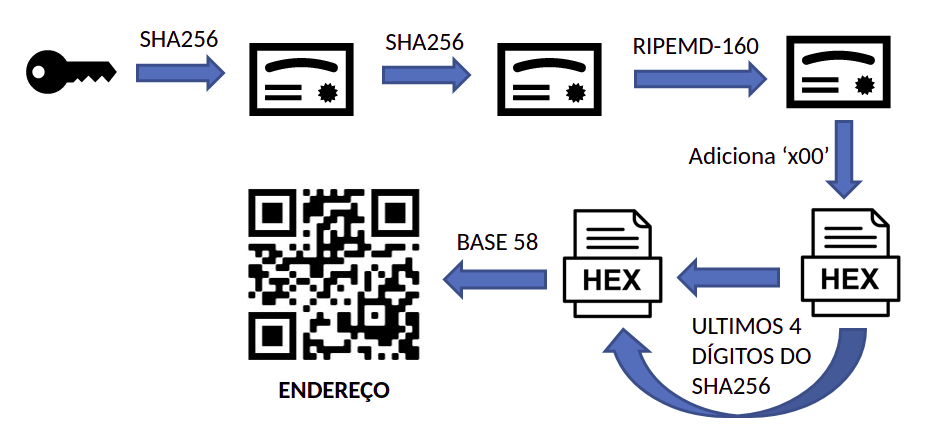
\includegraphics[width=0.9\textwidth]{imagens/fluxo_endereco}
	\caption{Fluxograma de geração do endereço}
	\label{fig:fluxo_endereco}
\end{figure}
%\clearpage

Em protocolos como o Bitcoin a chave pública não é divulgada fora das \textit{wallets}, em decorrência da possibilidade de, no futuro, a utilização do Algoritmo de Shor permita a obtenção da chave privada a partir da chave pública \cite{Mavroeidis2018}. 

Ainda que um computador quântico com \textit{\glspl{qubit}} suficientes para o processamento de um algoritmo de fatoramento de grandes números ainda não esteja no horizonte, a solução utilizada no Bitcoin pode implicar na resistência a tal brecha no futuro e foi adotada neste trabalho. 

\subsection{UTXO (Unspent Transactions Output)}

O Saldo de Transações Não-Gasto (UTXO) é uma lista, composta por todos os endereços registrados na rede, seu saldo atual e uma lista interna contendo todas as transações em que aquele endereço foi parte, seja de entrada ou saída. A lista é produzida a partir do processamento das transações existentes nos blocos, permitindo uma leitura mais simples dos saldos, sem a necessidade de procurar cada uma das transações nos blocos.

\subsection{Assinatura por delegação}

Assim como as chaves, o endereço identifica os usuários em uma rede \textit{blockchain}, mas, no caso especifico deste trabalho, também identifica as urnas, permitindo que os eleitores transfiram seus saldos de votos para elas, permitindo que as urnas assinem as cédulas virtuais de votação no momento da coleta dos votos, desta forma as urnas recebem a delegação dos usuários para assinarem as cédulas, ocultando os dados dos votantes.

\subsection{Bloco Registros}

Os blocos registros são blocos que contém as transações de criação de endereços, funcionando de forma similar a um banco de dados contendo endereços de todos os participantes da rede, incluindo ID dos eleitores, mesários e urnas (gerados a partir do algoritmo UUID4), nomes dos eleitores, apelidos e números dos candidatos. 

\subsection{Cédula}
É a abstração de uma cédula em papel, contendo campos específicos para assinatura (produzida pela urna) e o endereço de destino, referente ao candidato votado.

\subsection{Requisição de votação}
É a transação pela qual o eleitor transfere para urna seu saldo no sistema, permitindo que a mesma requeira uma cédula para que o eleitor registre seu voto. A requisição de votação também funciona como prova de comparecimento do usuário. 

\subsection{Bloco Produtos de Votação}

É o resultado da votação, produzido pelas urnas e contém as transações de transferências dos saldos dos eleitores para as urnas (uma unidade por vez) e das urnas para os candidatos, conforme votação.

\section{RDVE Wallet}

O primeiro aplicativo, desenvolvido em linguagem \textit{Dart} utilizando-se o \textit{framework Flutter} foi o \textit{\gls{wallet}} RDVE Wallet\footnote{Código fonte disponível em \url{https://github.com/rammyres/rdve_wallet}}, que permite a identificação do usuário no sistema. 

O aplicativo possui um módulo principal, capaz de gerar e gerenciar chaves criptográficas que identificam o usuário. 

\begin{figure}[!h]
	\centering
	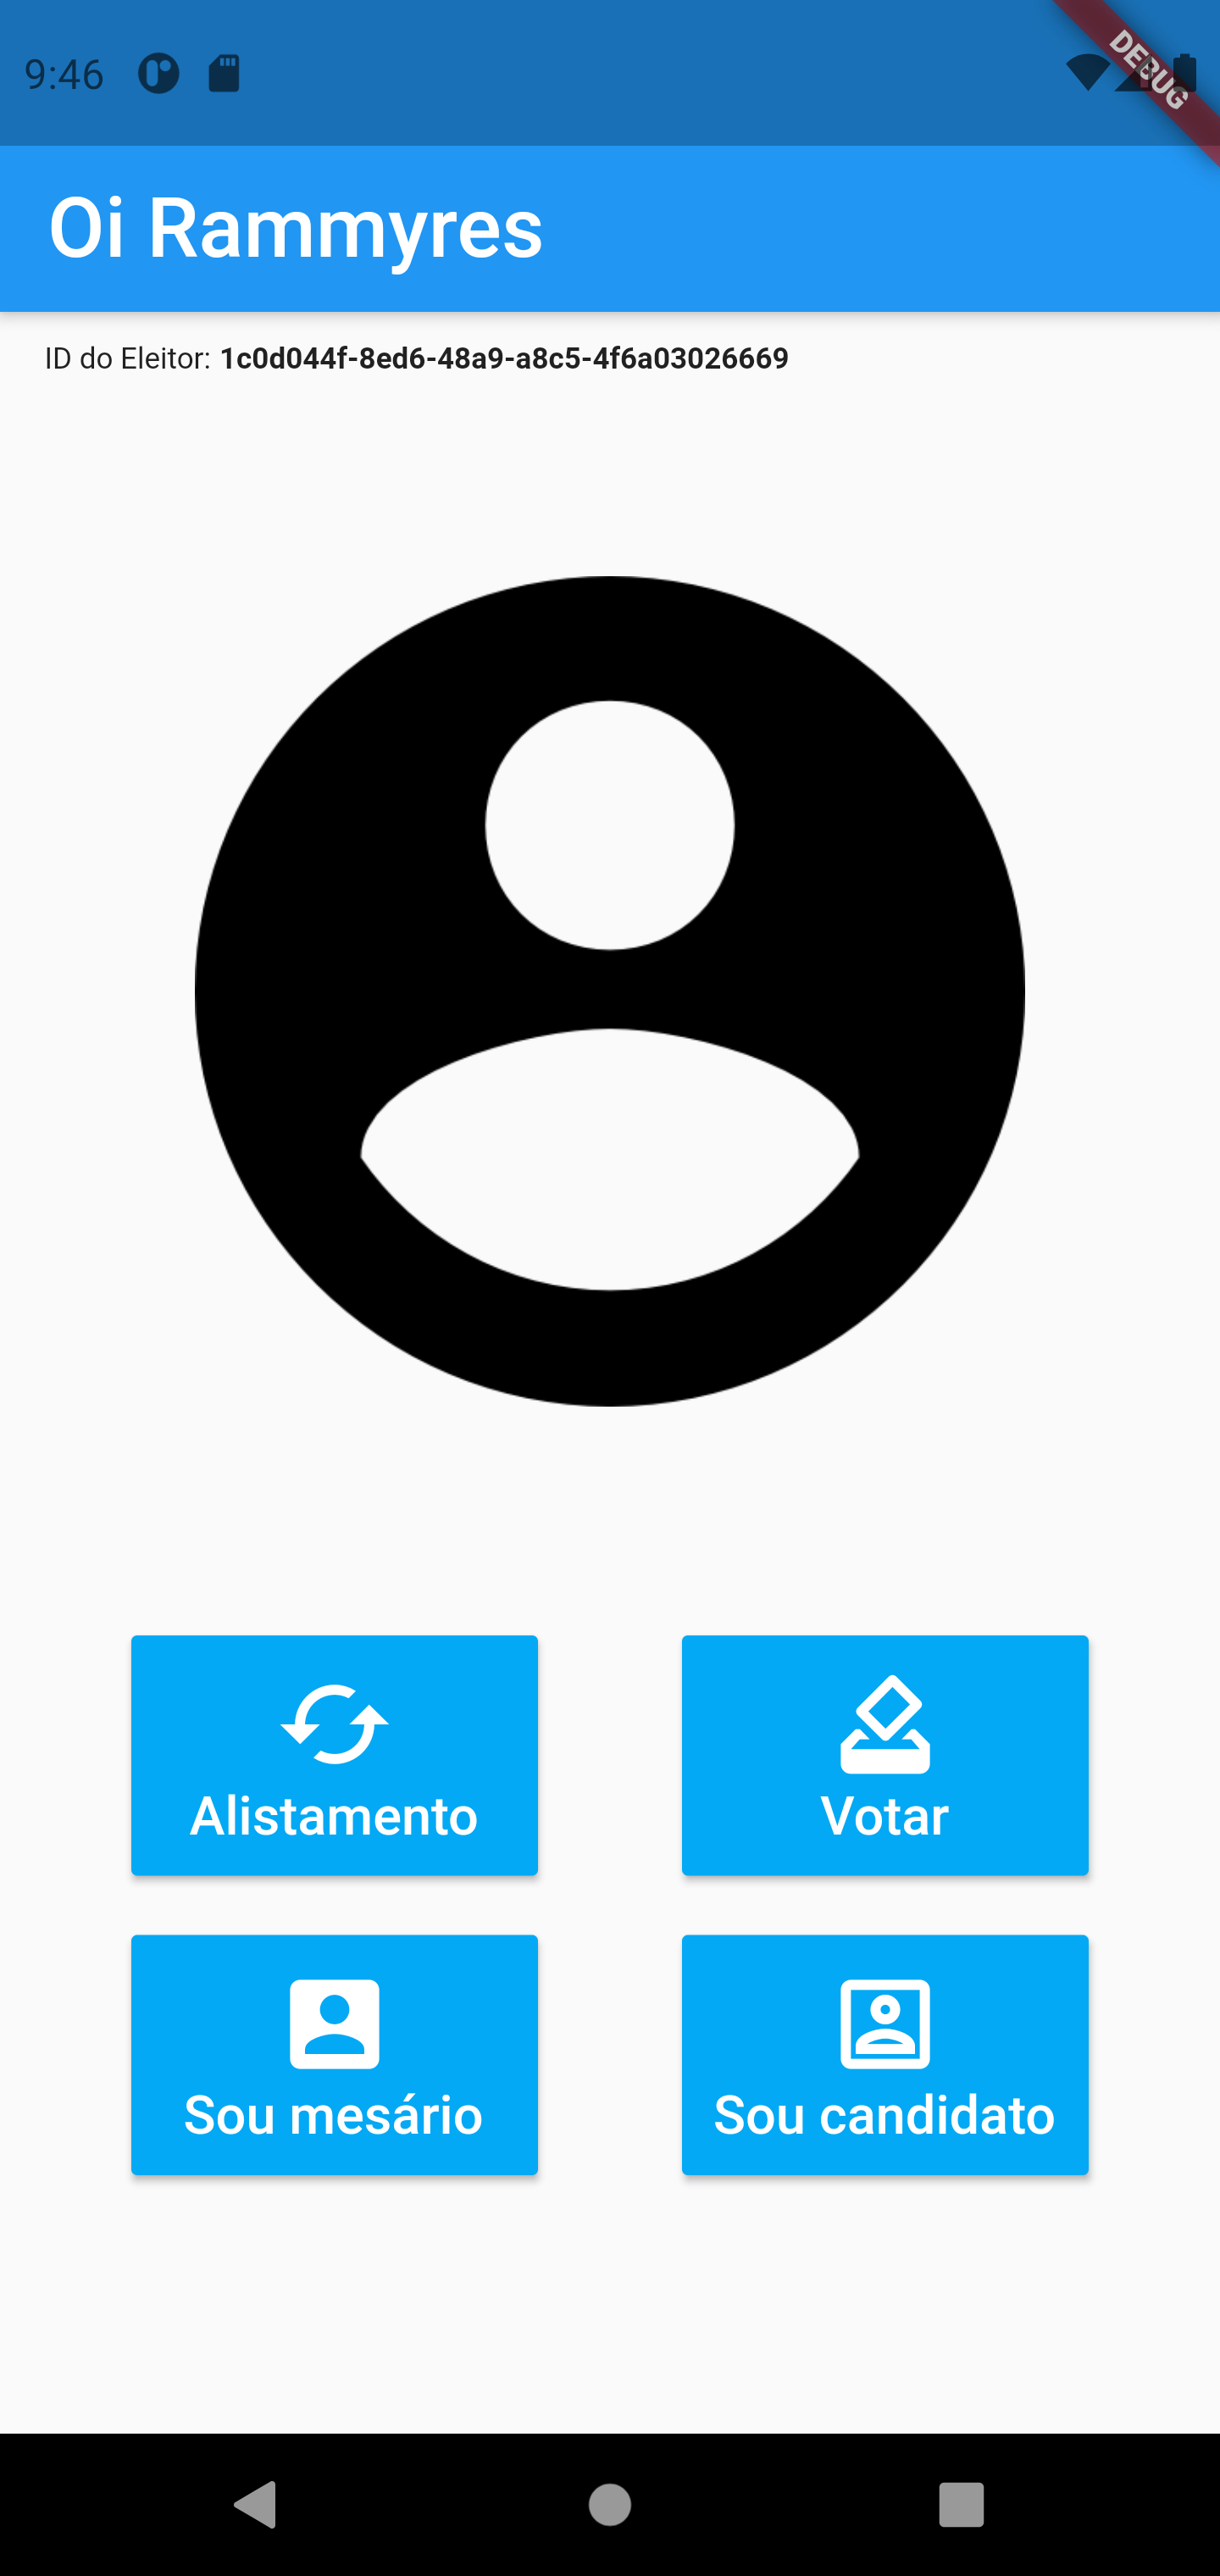
\includegraphics[width=0.5\textwidth]{imagens/wallet1}
	\caption{Módulo principal do RDVE Wallet}
	\label{fig:wallet1}
\end{figure}
\clearpage


A ID do eleitor identifica o mesmo dentro de todo o sistema, inclusive quado o mesmo se candidatar a cargo eletivo. Uma vez registrado no sistema o usuário pode requerer seu alistamento como eleitor, utilizado o módulo alistamento do aplicativo RDVE Coleta. Os dados são codificados como um objeto \gls{json}, contendo os dados necessários ao registro do usuário e apresentados como um \gls{qr1} que pode ser lido por outros dispositivos de modo \textit{offline}. 

\begin{figure}[!htb]
	\centering
	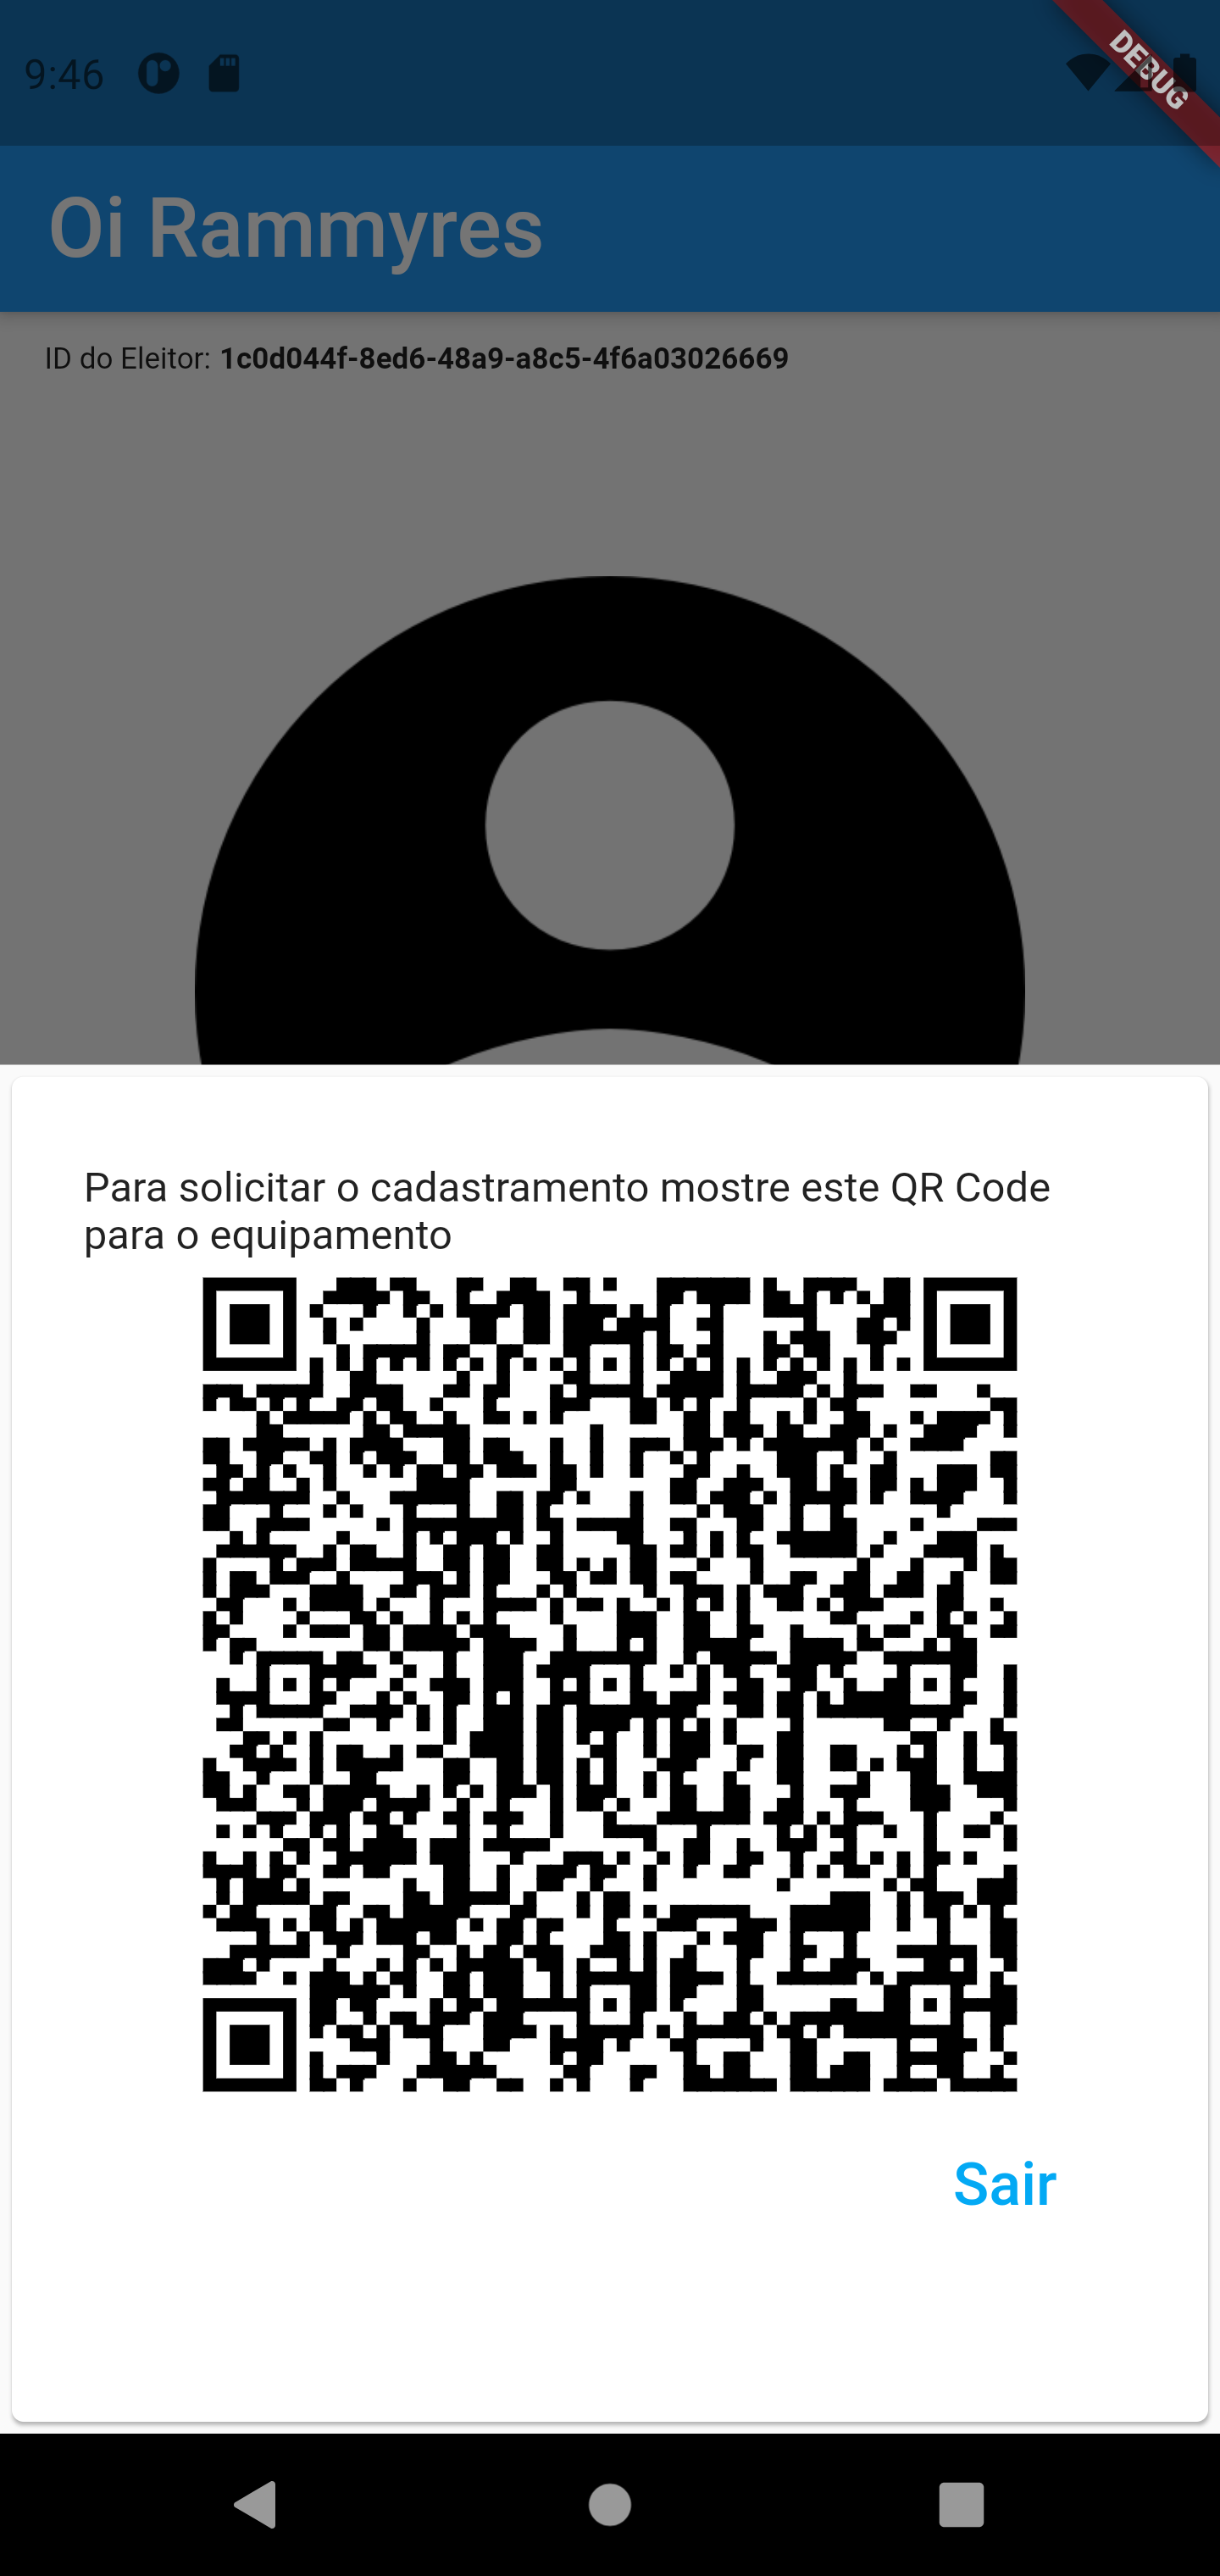
\includegraphics[width=0.5\textwidth]{imagens/wallet2}
	\caption{Módulo de alistamento}
	\label{fig:wallet2}
\end{figure}

De forma similar, existem módulos para registro como operador de urna (mesário) e candidatura. No primeiro caso não há geração de novas chaves criptográficas. 

\begin{figure}[!htb]
\centering
\begin{minipage}{0.47\textwidth}%	
	\centering
	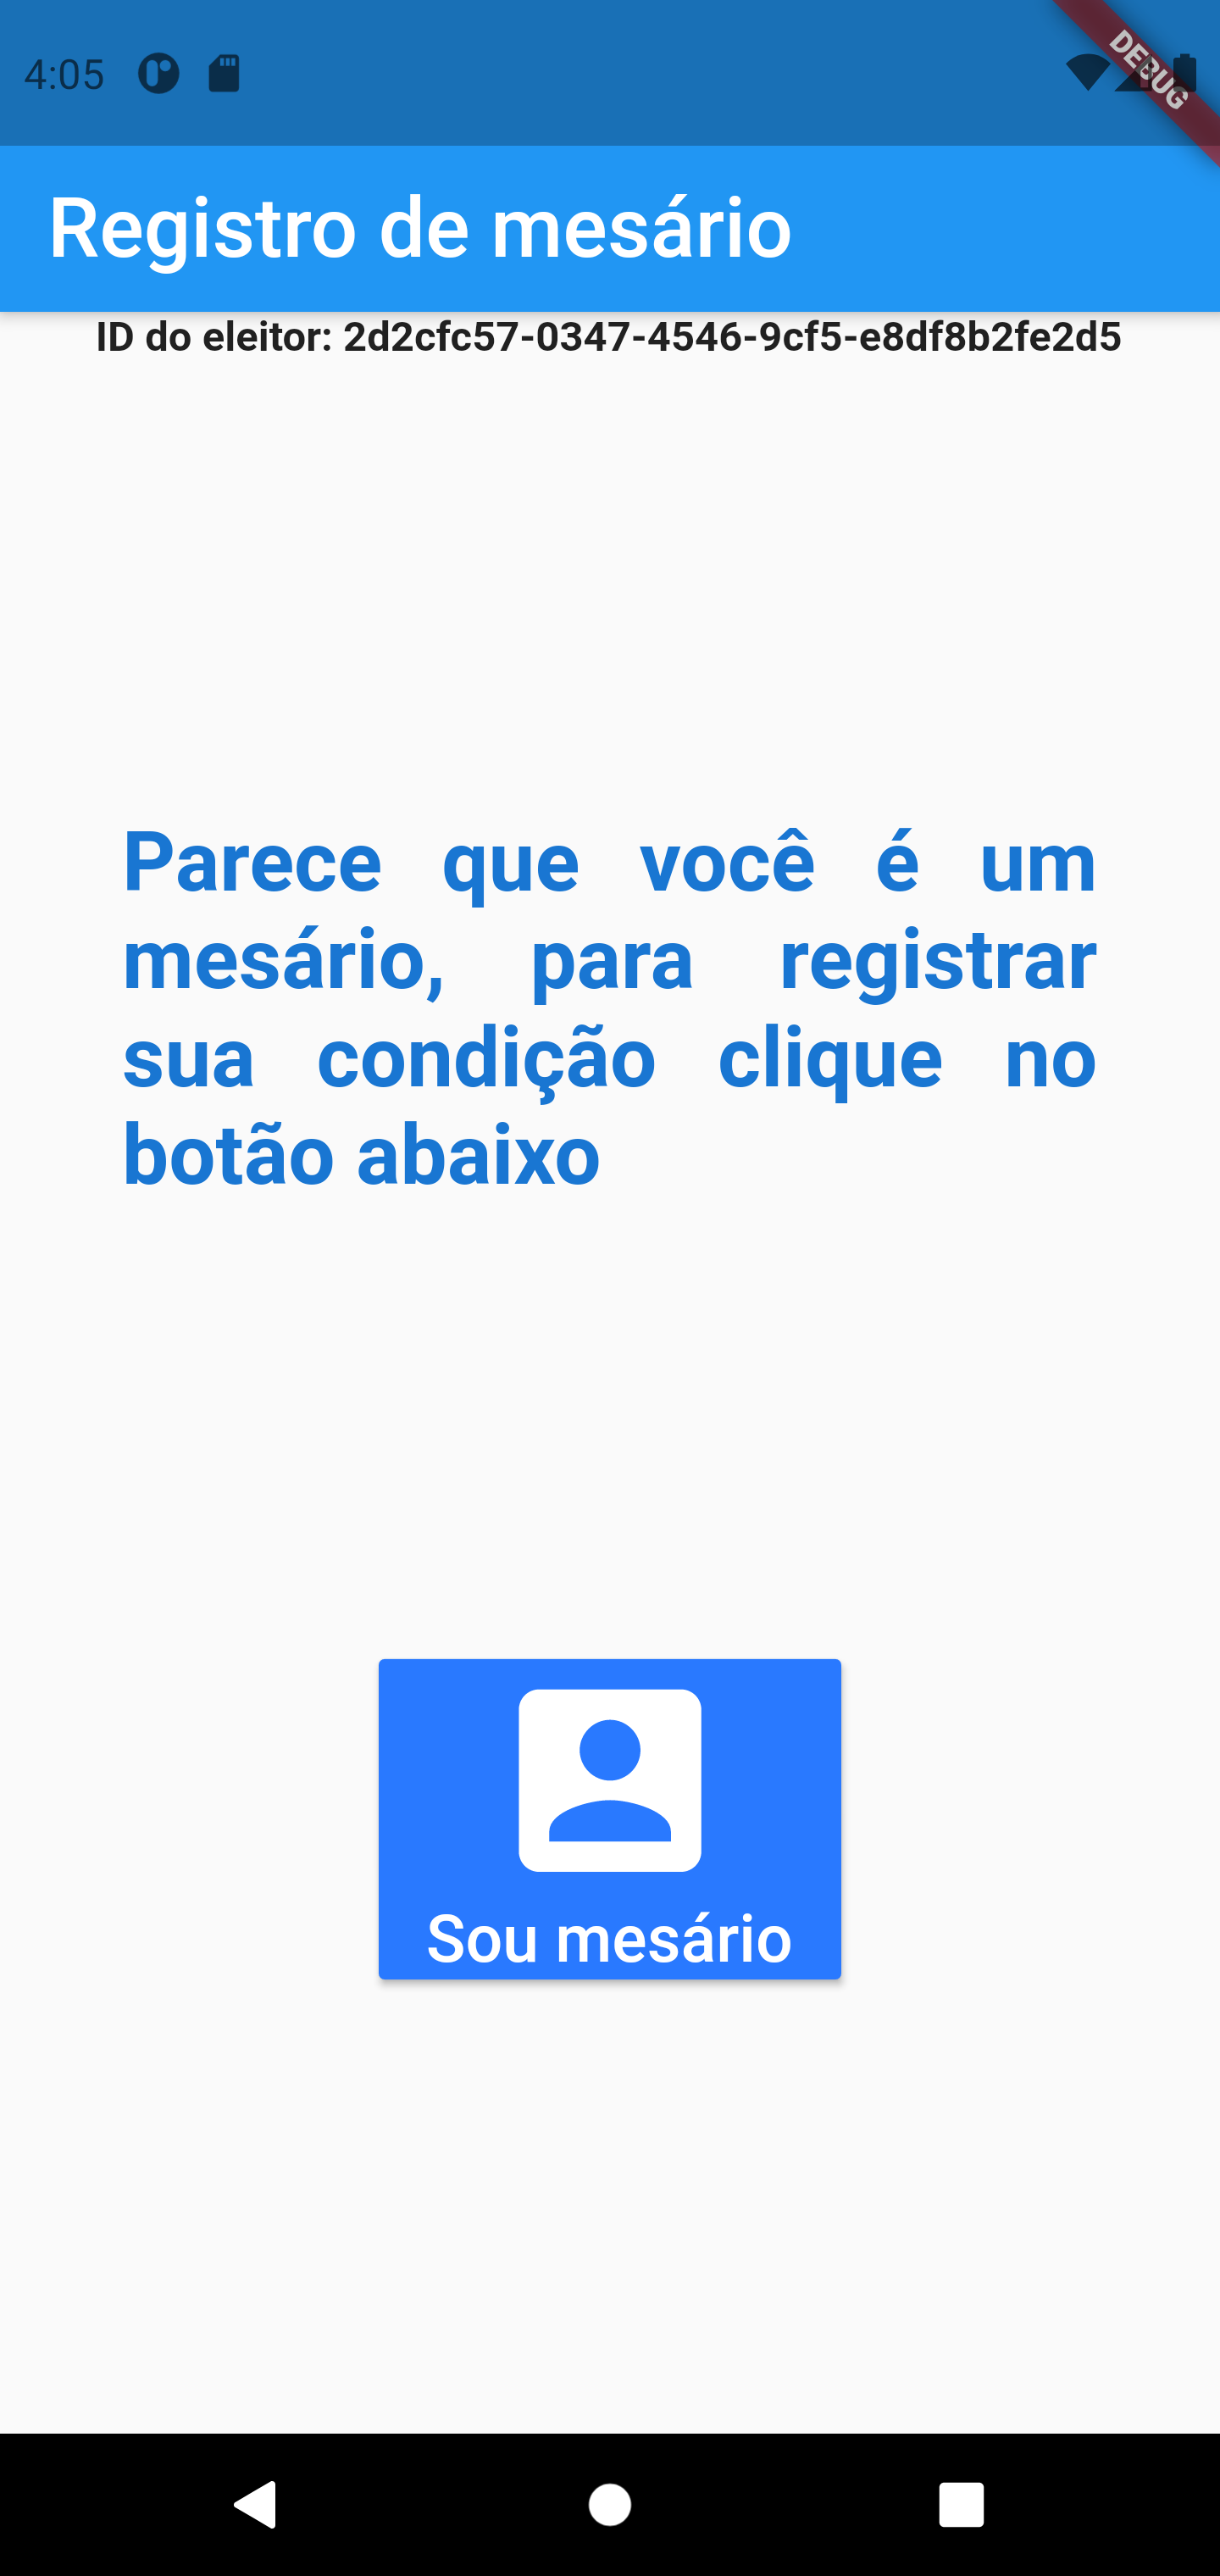
\includegraphics[width=.9\textwidth]{imagens/wallet_mesario}
	\caption{Módulo de registro do operador de urna}
	\label{fig:wallet_mesario}
\end{minipage}
\hfill
\begin{minipage}{0.47\textwidth}%
	\centering
	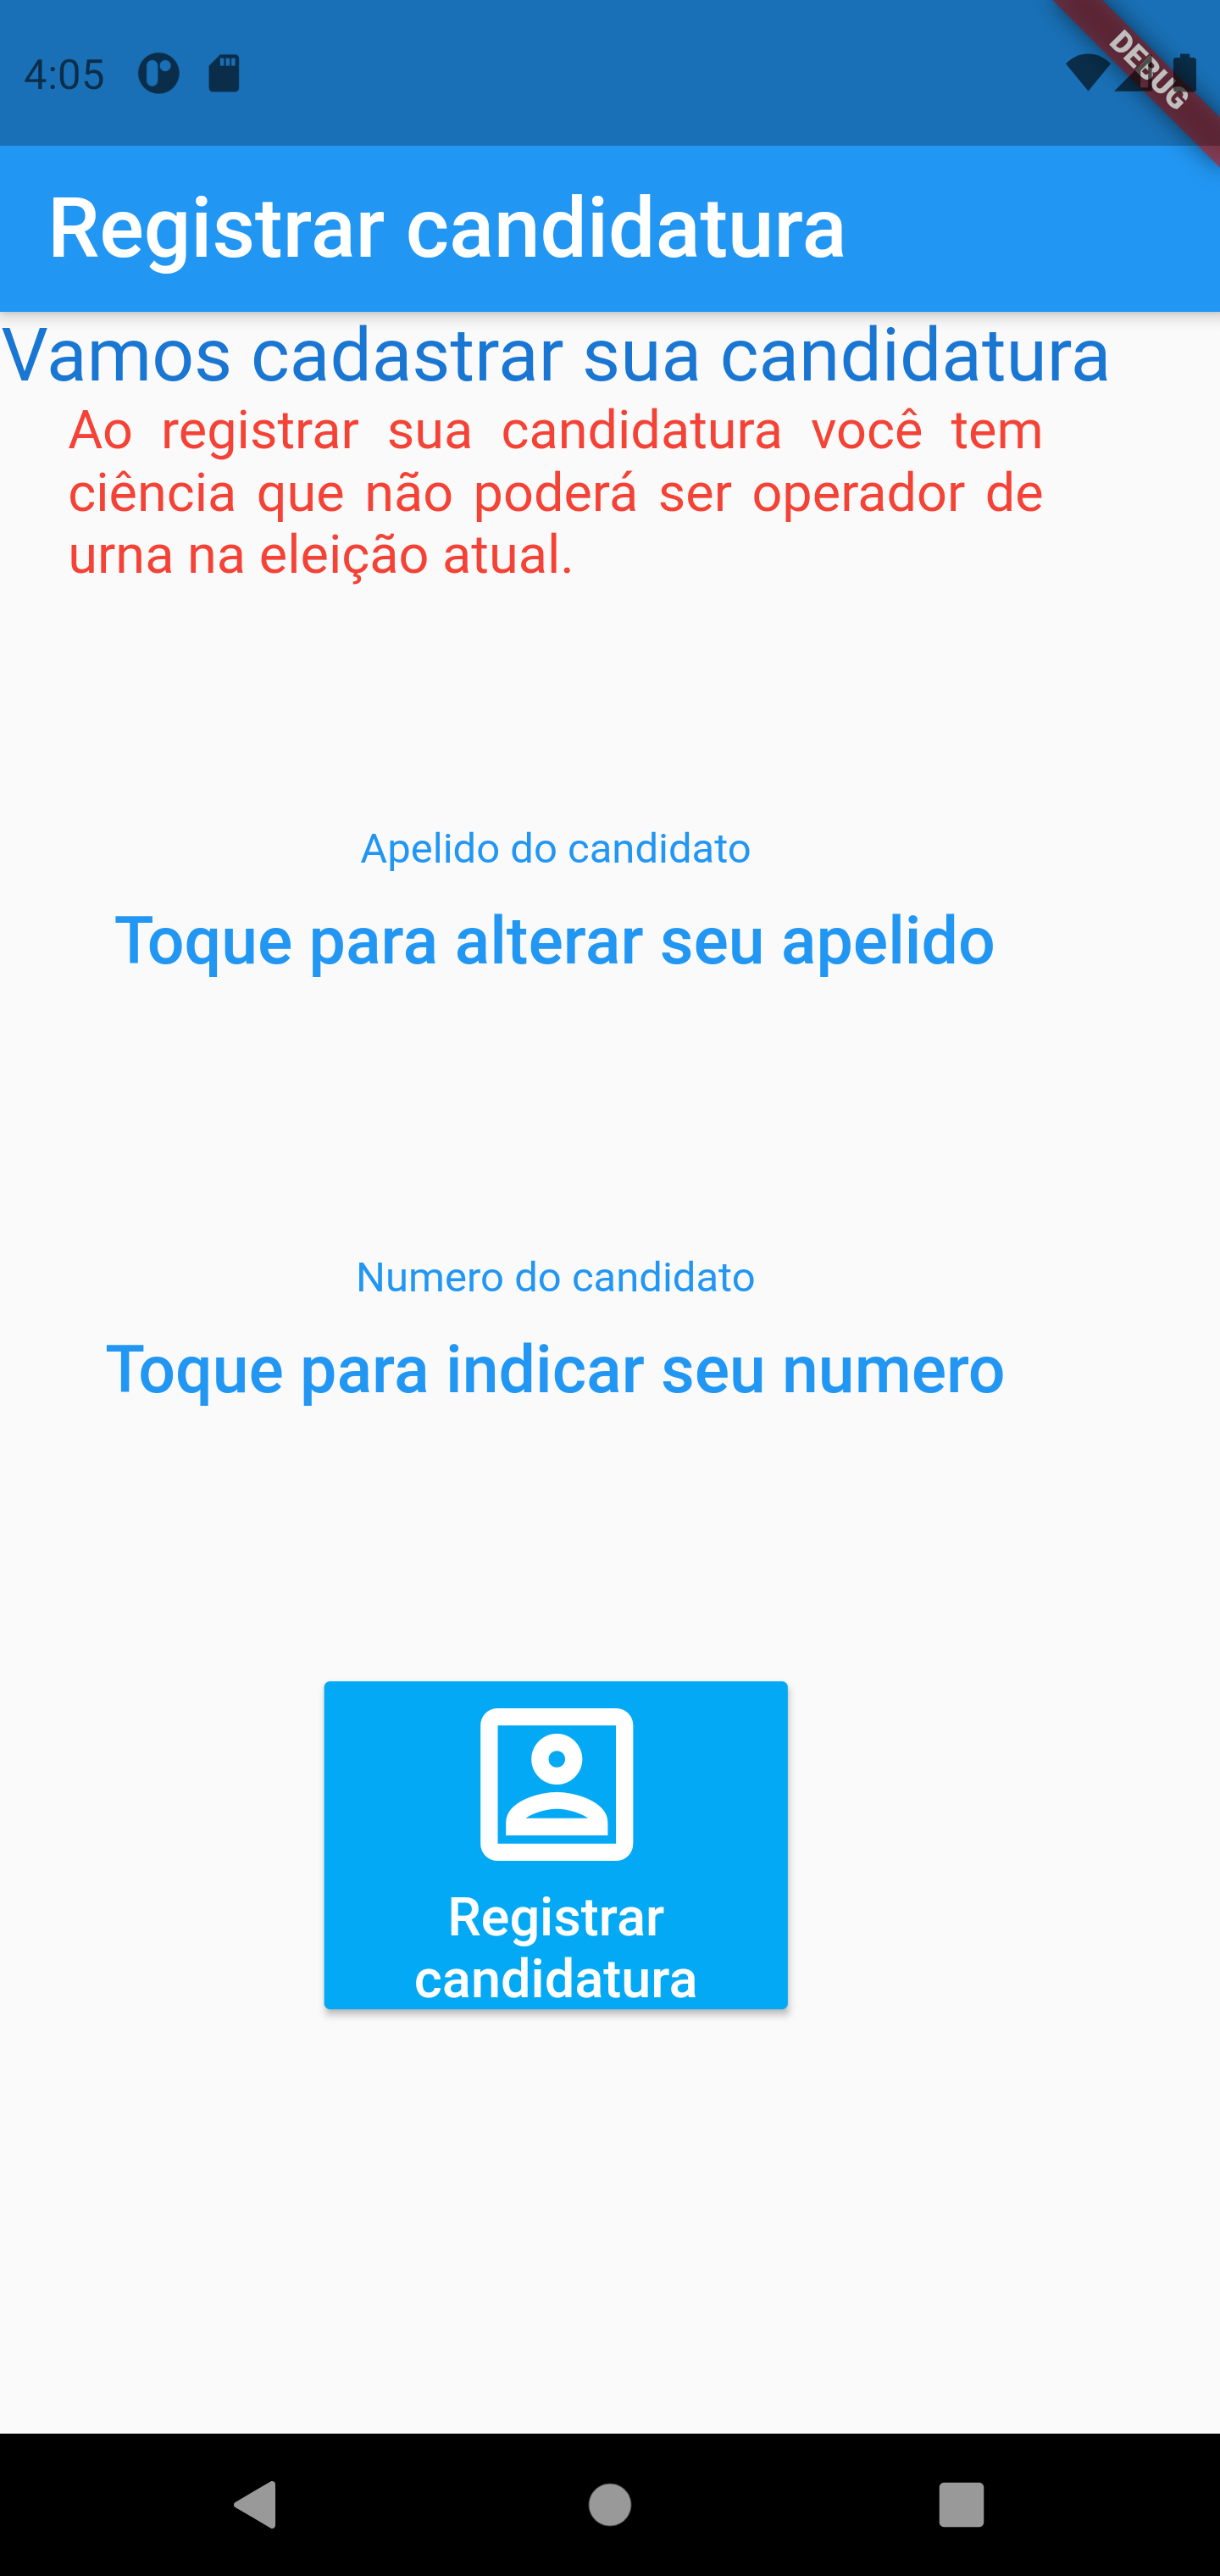
\includegraphics[width=.9\textwidth]{imagens/wallet_candidatura}
	\caption{Módulo de registro de candidatura}
	\label{fig:wallet_candidato}
\end{minipage}
\end{figure}
\clearpage

A comunicação com o sistema de coleta utiliza o mesmo princípio, gerando \glspl{qr1} contendo os dados necessários ao cadastramento de operadores e candidatos. 

Por fim o módulo de operação de urna permite que o mesário libere o alistamento eleitoral, o registro de candidatura e o voto. 

\begin{figure}[!htb]
	\centering
	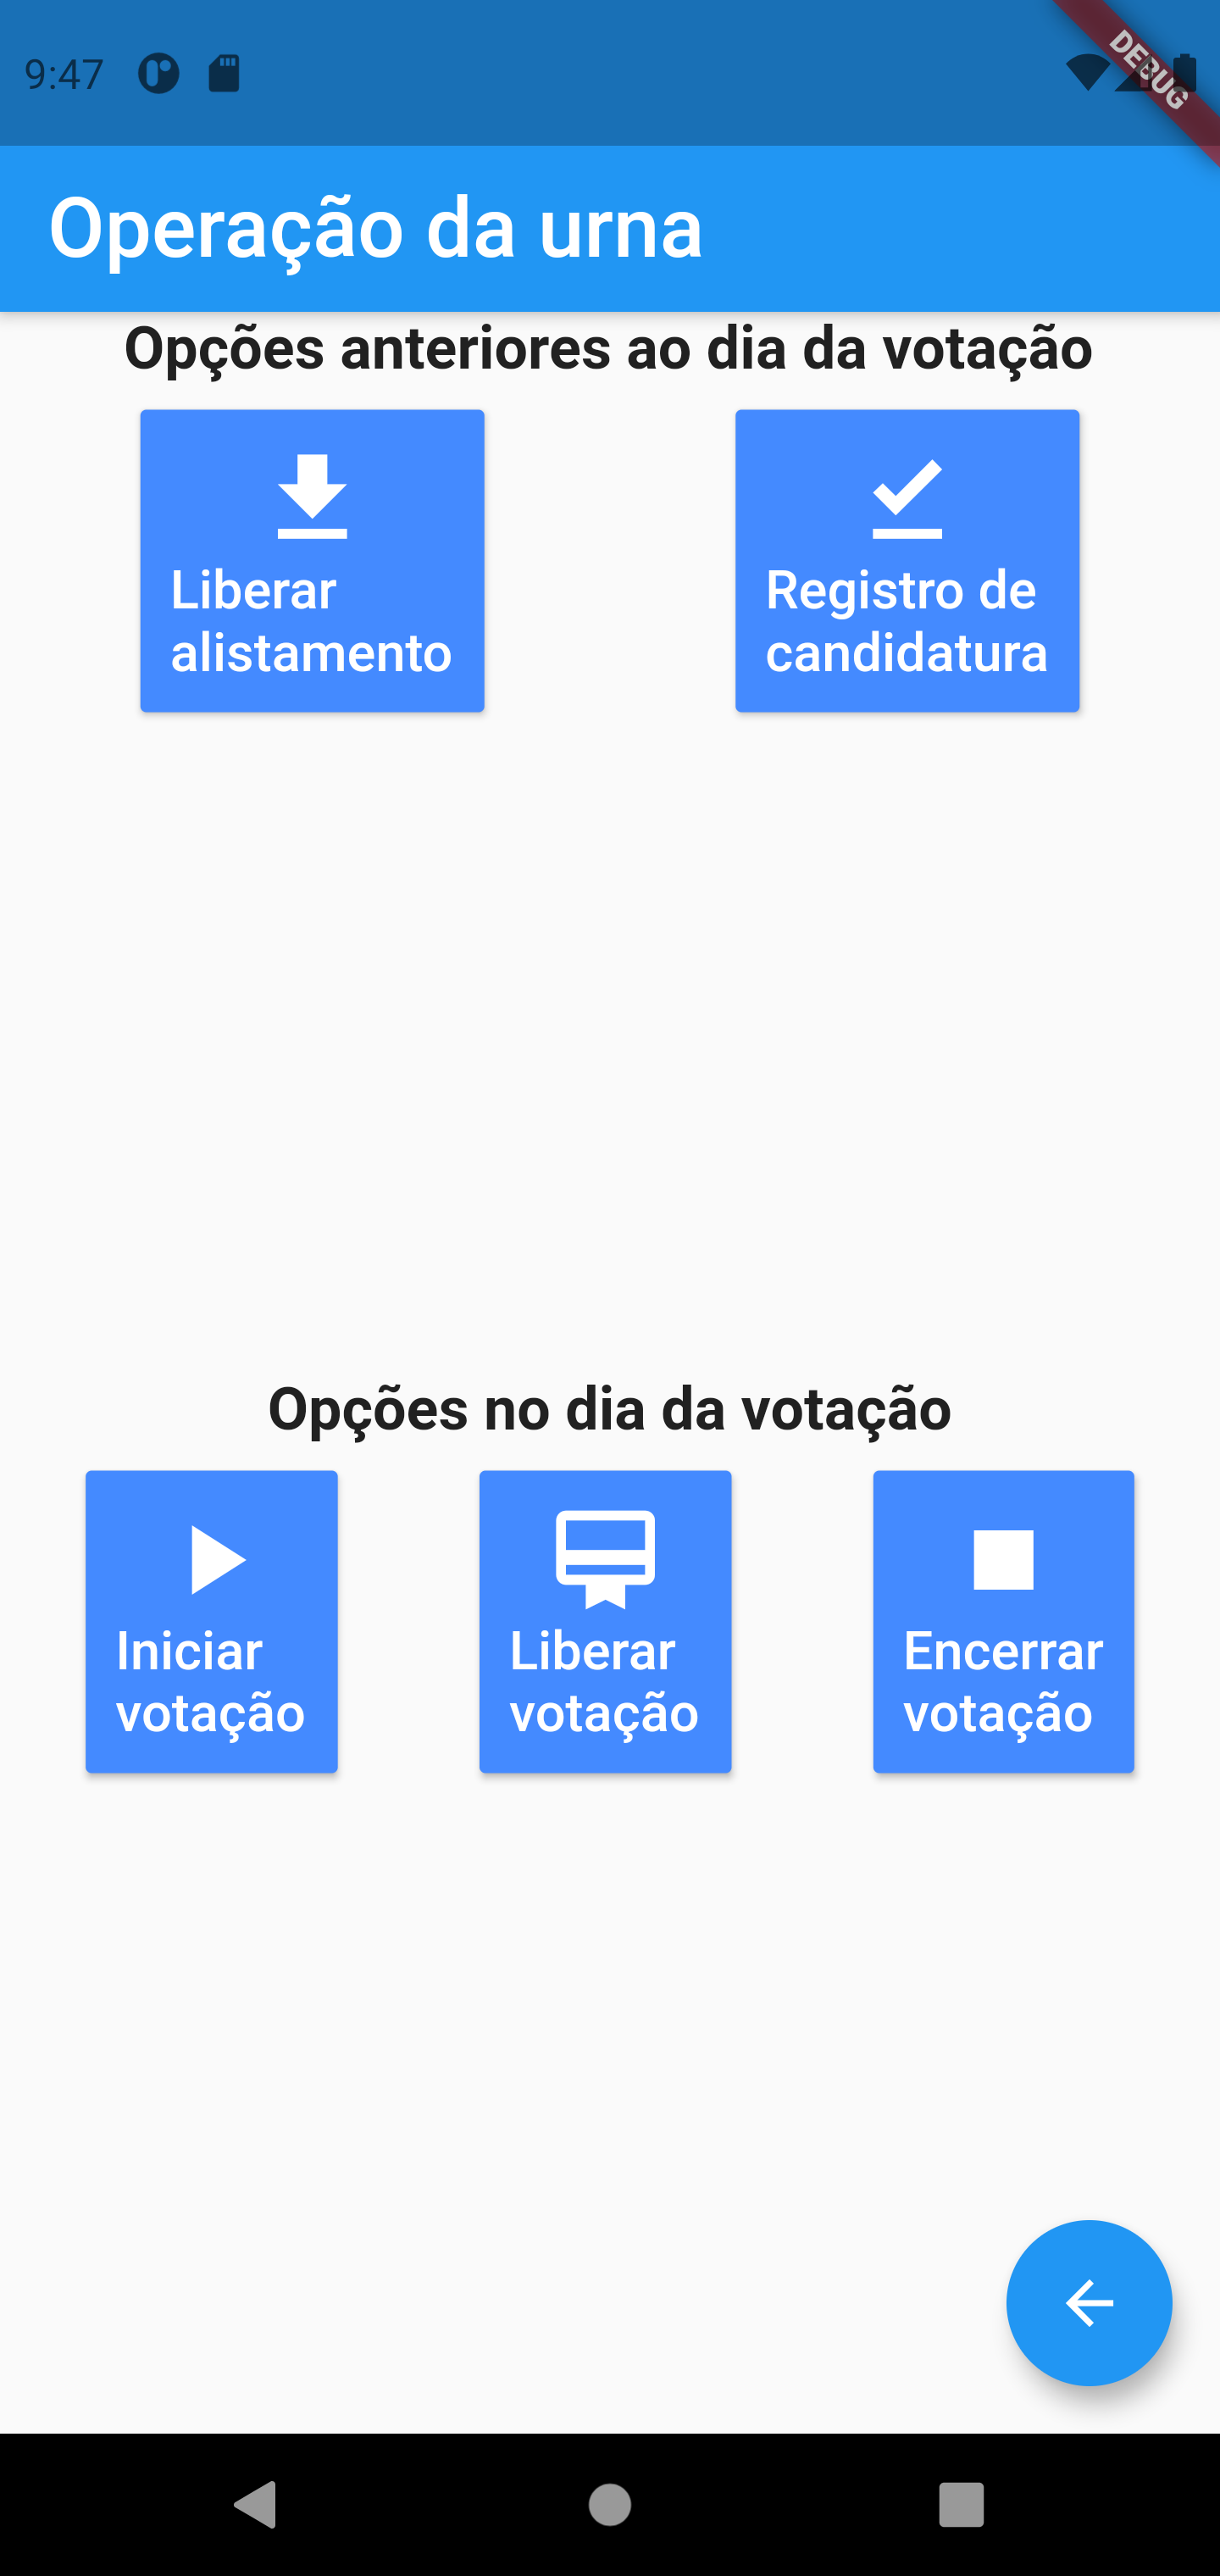
\includegraphics[width=0.5\textwidth]{imagens/wallet3}
	\caption{Módulo de operação das urnas}
	\label{fig:wallet_operador}
\end{figure}
\clearpage

\section{RDVE Coleta}

O RDVE Coleta\footnote{Código fonte disponível em \url{https://github.com/rammyres/rdve_coleta}} foi projetado em Python como um amalgama de dois projetos separados, o RDVE Coleta em si e o RDVE Urna.

\begin{figure}[h!]
	\centering
	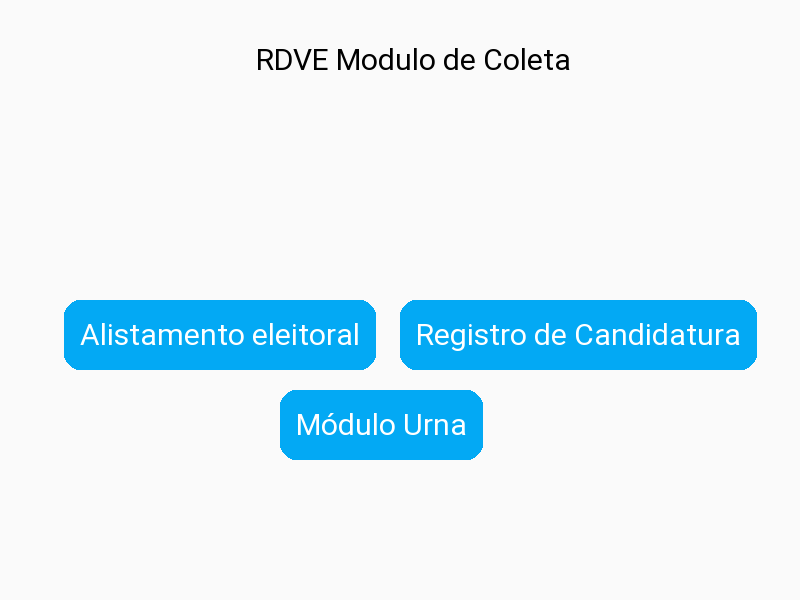
\includegraphics[width=0.8\textwidth]{imagens/coleta1}
	\caption{Sistema RDVE Coleta}
	\label{fig:coleta1}
\end{figure}

O RDVE Coleta registra eleitores e candidatos, bem como as requisições de votação, cédulas e os produtos de votação. Cada voto registrado na urna é procedido por uma aleatorização da lista de cédulas e somente ao final os votos, novamente embaralhados, tem seus \glspl{hash1} incluídos na \gls{merkle}, impedindo que se possa recuperar a ordem de votação por meios indiretos. 

\clearpage

\begin{figure}[!h]
	\centering
	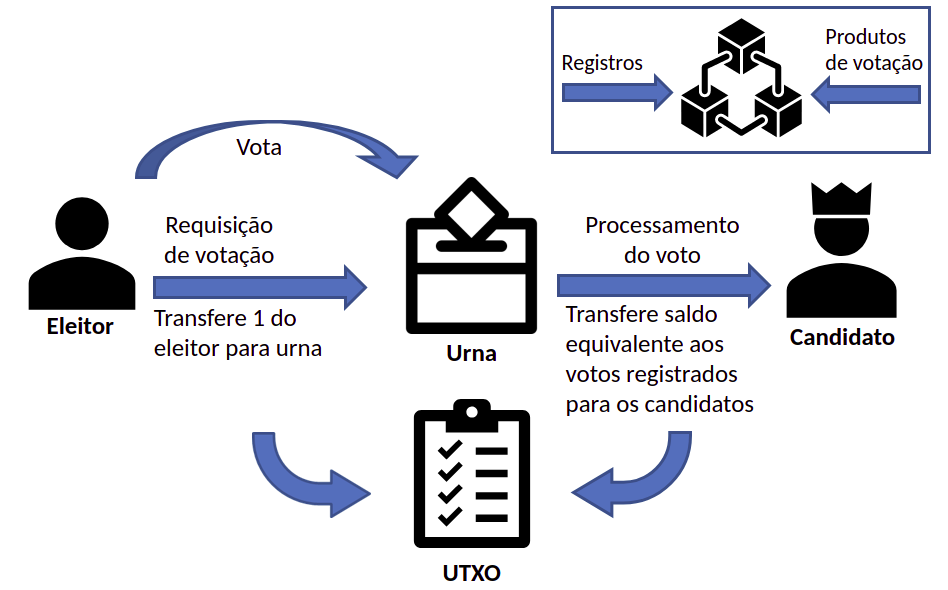
\includegraphics[width=0.9\textwidth]{imagens/fluxo_dados}
	\caption{Fluxo dos dados no sistema RDVE Coleta}
	\label{fig:fluxo_dados}
\end{figure}


\section{Resultados Obtidos}

A partir da execução dos aplicativos descritos foi possível realizar votações simuladas sem participações de terceiros, em decorrência da pandemia mundial de COVID-19.

Os registros representaram os dados inseridos e, em decorrência da forma de representação, mantiveram-se fidedignos e foi possível recuperar os estados registrados através da persistência dos objetos descritos acima como texto em formato \gls{json}. Os arquivos de registro e produtos de votação compreendiam blocos íntegros e todos os seus registros tinham entradas em sua \glspl{merkle} que podiam ter provas efetivamente produzíveis. 

Nas simulações não foi possível recuperar a ordem da votação ou cruzar o voto com o eleitor que o produziu. Em inspeção manual também foi possível verificar que o UTXO tinha saldos compatíveis com as transações existentes nos blocos de produtos de votação. 